%=========================================================
\chapter{Simulation-Based Swaption Pricing and Second-Stage Calibration}
\label{chap:pricing_methodology}
%=========================================================

Having established in Chapter~\ref{chap:sim_comparison} that the stable latent-factor
model produces well-behaved simulated paths, this chapter develops the full pricing and
calibration framework. Section~\ref{sec:bachelier_model} describes the Bachelier normal
model and its two roles in the pipeline: as a pricing-target converter in the second-stage
calibration and as an implied-volatility inverter for reporting.
Section~\ref{sec:bachelier_greeks} collects the analytic Greeks of the Bachelier price.
Section~\ref{sec:second_stage_calibration} presents the second-stage calibration
procedure. Section~\ref{sec:pricing_diagnostics} summarises the pricing diagnostics.

%=========================================================
\section{The Bachelier Normal Swaption Pricing Model}
\label{sec:bachelier_model}
%=========================================================

A European payer swaption with option expiry $T_e$ and swap tenor $T_s$ gives the
holder the right to enter a fixed-for-floating swap at expiry. Under the
\emph{annuity measure} $\mathbb{Q}^A$, the forward swap rate $F(t)$ is a martingale.
In the Bachelier (normal) model \citep{Bachelier1900}, it evolves as
\begin{equation}
    dF(t) = \sigma\, dW^A(t),
    \label{eq:bachelier_sde}
\end{equation}
where $\sigma > 0$ is the \emph{normal volatility}. This model accommodates negative
rates and has been the standard EUR swaption quotation convention since 2014.

Under~\eqref{eq:bachelier_sde} the time-$0$ price of a payer swaption (notional $N$,
strike $K$) is
\begin{equation}
    V^{\mathrm{pay}}
    =
    N \cdot A(0) \cdot
    \Bigl[
        (F_0 - K)\,\Phi(d)
        +
        \sigma\sqrt{T_e}\,\phi(d)
    \Bigr],
    \qquad
    d = \frac{F_0 - K}{\sigma\sqrt{T_e}},
    \label{eq:bachelier_payer}
\end{equation}
where $\Phi$ and $\phi$ are the standard normal CDF and PDF, $F_0=F(0)$ is the
time-$0$ forward swap rate, and $A(0)=\sum_{j=1}^{n}\Delta\,P(0,T_e+j\Delta)$ is the
annuity. For an at-the-money swaption ($K=F_0$, $d=0$):
\begin{equation}
    V^{\mathrm{ATM}}
    =
    N \cdot A(0) \cdot \frac{\sigma\sqrt{T_e}}{\sqrt{2\pi}}.
    \label{eq:bachelier_atm}
\end{equation}

\paragraph{Two roles of the Bachelier formula.}
The Bachelier formula serves \emph{two distinct roles} in the implementation and they
should not be confused.

\begin{enumerate}
    \item \textbf{Pricing target for the second-stage calibration.}
    Market data are distributed as ATM normal volatilities
    $\sigma^{(i)}_{\mathrm{mkt}}$ (in basis points). These are converted to prices via
    the ATM formula~\eqref{eq:bachelier_atm}:
    \begin{equation}
        V^{(i)}_{\mathrm{mkt}}
        =
        N \cdot A^{(i)}_0 \cdot
        \frac{\sigma^{(i)}_{\mathrm{mkt}}\,\sqrt{T_e^{(i)}}}{\sqrt{2\pi}}.
        \label{eq:stage2_target}
    \end{equation}
    This is a \emph{fixed, non-differentiable target} computed once per observation from
    the time-$0$ annuity $A_0$ (decoded at the first-stage latent state). The model MC
    price $\hat{V}_{\mathrm{MC}}$ is then trained to match it.

    \item \textbf{Implied-volatility inversion for reporting.}
    After pricing, the MC price is inverted back to a normal implied volatility for
    comparison with market quotes:
    \begin{equation}
        \hat{\sigma}_{\mathrm{mod}}
        =
        \frac{\hat{V}_{\mathrm{MC}} \cdot \sqrt{2\pi}}{N \cdot A(0) \cdot \sqrt{T_e}}.
        \label{eq:implied_vol}
    \end{equation}
    For off-ATM strikes the inversion uses Brent's method
    (\texttt{implied\_bachelier\_vol()} in \texttt{pricing.py}). Reporting in basis-point
    vol space makes model errors directly comparable to market-convention bid--ask
    spreads.
\end{enumerate}

\paragraph{Monte Carlo price.}
The model-implied swaption price is estimated by
\begin{equation}
    \hat{V}^{\mathrm{pay}}_{\mathrm{MC}}
    =
    \frac{1}{M}
    \sum_{m=1}^{M}
    D^{(m)}_{T_e} \cdot A^{(m)}_{T_e} \cdot
    \max\!\bigl(F^{(m)}_{T_e} - K,\; 0\bigr),
    \label{eq:mc_price}
\end{equation}
where $D^{(m)}_{T_e}=\exp(-\sum_{k=0}^{n_e-1}\tfrac{r^{(m)}_k+r^{(m)}_{k+1}}{2}\,\Delta t)$
is the pathwise trapezoidal money-market discount factor, and $A^{(m)}_{T_e}$,
$F^{(m)}_{T_e}$ are the annuity and forward swap rate decoded from the bond curve at
expiry. Implemented in \texttt{swaption\_mc\_price\_from\_simulation()}.

%=========================================================
\section{Analytic Greeks in the Bachelier Model}
\label{sec:bachelier_greeks}
%=========================================================

The following proposition collects the closed-form sensitivities of the Bachelier payer
price~\eqref{eq:bachelier_payer}.

\begin{proposition}[Bachelier Greeks]
\label{prop:bachelier_greeks}
Let $V=V^{\mathrm{pay}}$ as in~\eqref{eq:bachelier_payer}. Define
$d=(F_0-K)/(\sigma\sqrt{T_e})$. Then:
\begin{align}
    \Delta  &= \frac{\partial V}{\partial F_0}         = N\!A\,\Phi(d),
    \label{eq:delta} \\
    \mathcal{V} &= \frac{\partial V}{\partial \sigma}  = N\!A\sqrt{T_e}\,\phi(d),
    \label{eq:vega} \\
    \Gamma  &= \frac{\partial^2 V}{\partial F_0^2}     = \frac{N\!A\,\phi(d)}{\sigma\sqrt{T_e}},
    \label{eq:gamma} \\
    \Theta  &= \frac{\partial V}{\partial T_e}         = \frac{N\!A\,\sigma\,\phi(d)}{2\sqrt{T_e}},
    \label{eq:theta} \\
    \mathrm{DV01} &= \Delta\times 10^{-4}              = \frac{N\!A\,\Phi(d)}{10\,000},
    \label{eq:dv01} \\
    \mathrm{Vanna} &= \frac{\partial^2 V}{\partial F_0\,\partial\sigma} = -\frac{N\!A\,\phi(d)\,d}{\sigma},
    \label{eq:vanna} \\
    \mathrm{Volga} &= \frac{\partial^2 V}{\partial\sigma^2}
                   = \frac{N\!A\sqrt{T_e}\,d^2\,\phi(d)}{\sigma}.
    \label{eq:volga}
\end{align}
For the receiver swaption, $\Delta^{\mathrm{rec}}=N\!A\,(\Phi(d)-1)=-N\!A\,\Phi(-d)$,
and all other Greeks are identical. Put-call parity:
$\Delta^{\mathrm{pay}}-\Delta^{\mathrm{rec}}=N\!A$.
\end{proposition}

\begin{proof}
Follows by direct differentiation of~\eqref{eq:bachelier_payer}. For Delta, the terms
involving $\phi(d)\cdot\partial d/\partial F_0$ cancel by construction of $d$. The
remaining Greeks use $\partial d/\partial\sigma=-d/\sigma$ and $\phi'(d)=-d\,\phi(d)$.
\end{proof}

\paragraph{ATM simplifications ($K=F_0$, $d=0$).}
Since $\Phi(0)=\tfrac{1}{2}$ and $\phi(0)=(2\pi)^{-1/2}$:
\begin{equation}
\Delta^{\mathrm{ATM}}  = \tfrac{1}{2}N\!A, \quad
\mathcal{V}^{\mathrm{ATM}} = N\!A\sqrt{T_e/(2\pi)}, \quad
\Gamma^{\mathrm{ATM}} = \tfrac{N\!A}{\sigma\sqrt{2\pi T_e}}, \quad
\Theta^{\mathrm{ATM}} = \tfrac{N\!A\,\sigma}{2\sqrt{2\pi T_e}}.
\label{eq:atm_greeks}
\end{equation}
Vanna and Volga vanish at the money. Note that $\mathcal{V}^{\mathrm{ATM}} =
\partial V^{\mathrm{ATM}}/\partial\sigma$, consistent with~\eqref{eq:bachelier_atm}.

\paragraph{Implementation.}
The analytic Greeks are in \texttt{bachelier\_greeks()} in \texttt{pricing.py}, which
returns a dict with keys \texttt{delta}, \texttt{vega}, \texttt{gamma}, \texttt{theta},
\texttt{dv01}, \texttt{vanna}, \texttt{volga}. Edge cases ($T_e\leq0$ or $\sigma\leq0$)
return intrinsic greeks with zero time-value components. The ATM identities and
put-call parity pass analytic verification (see \texttt{test\_greeks.py}).

\paragraph{Theta--Gamma identity.}
A useful self-consistency check follows from combining~\eqref{eq:gamma}
and~\eqref{eq:theta}:
\begin{equation}
    \Theta = \tfrac{1}{2}\,\sigma^2\,\Gamma\,(\sigma\sqrt{T_e}).
    \label{eq:theta_gamma}
\end{equation}
This is the Bachelier analogue of the Black--Scholes Theta--Gamma relation.  It can be
verified on any model-implied swaption as a diagnostic: if the MC-implied $\Theta$ and
$\Gamma$ (obtained by finite differences) violate~\eqref{eq:theta_gamma}, the model
simulation is internally inconsistent.

%=========================================================
\section{Second-Stage Calibration}
\label{sec:second_stage_calibration}
%=========================================================

\subsection{Calibration Objective}
\label{subsec:calib_objective}

For each market ATM swaption quote $(\sigma^{(i)}_\mathrm{mkt}, T_e^{(i)}, T_s^{(i)},
t^{(i)})$, the fixed target is $V^{(i)}_\mathrm{mkt}$ from~\eqref{eq:stage2_target}.
The mini-batch stage-2 loss is
\begin{equation}
    \mathcal{L}_2(\Omega_2)
    =
    \frac{1}{|\mathcal{B}|}
    \sum_{i \in \mathcal{B}}
    \bigl(
        10\,000\cdot(\hat{V}^{(i)}_\mathrm{MC} - V^{(i)}_\mathrm{mkt})
    \bigr)^2
    +
    \lambda_G \!\sum_{p \in \mathcal{G}} \lVert p - p_0 \rVert^2
    +
    \lambda_K \lVert N_K - N_{K,0} \rVert^2.
    \label{eq:stage2_loss}
\end{equation}
The factor $10\,000$ re-scales prices to basis-point units for numerical conditioning.
The L$^2$ penalties keep the decoder $\mathcal{G}$ and the drift intercept $N_K$ close
to their first-stage values. Implemented in \texttt{calibrate\_second\_stage()} and
\texttt{swaption\_price\_loss\_single()}.

\subsection{Trainable Parameter Groups}
\label{subsec:param_groups}

\begin{itemize}
    \item \textbf{$\mathcal{H}$ (always, full lr $\eta$)}: the diffusion network controls
    the volatility of simulated paths and is the primary lever for fitting the vol surface.
    \item \textbf{$\mathcal{G}$ (optional, lr $0.1\eta$, regularised)}: small decoder
    updates adjust the forward curve at expiry.
    \item \textbf{$K.N$ (optional, lr $0.1\eta$, regularised)}: allows the
    mean-reversion equilibrium $z^*=-M^{-1}N$ to shift without breaking the
    Hurwitz constraint (K.V is always frozen).
    \item \textbf{Encoder, K.V, $\mathcal{R}$ frozen}: reconstruction quality and
    stable simulation properties are preserved.
\end{itemize}

\subsection{Variance Reduction and Gradient Flow}
\label{subsec:antithetic}

\emph{Antithetic variates}: the $M/2$ pre-drawn noise realisations $\varepsilon$ and
$-\varepsilon$ are paired, halving MC variance and ensuring half the paths are always
in-the-money.

\emph{Reparameterisation}: the Euler step
$z_{t+1}=z_t+\mu(z_t)\Delta t + L(z_t;\mathcal{H})\varepsilon_t\sqrt{\Delta t}$
is a deterministic function of the fixed noise, so gradients flow through
$L(z_t;\mathcal{H})$ at every step. The discount $D_{T_e}$ is computed under
\texttt{no\_grad()} via the frozen $\mathcal{R}$.

Per-group gradient clipping: $\mathcal{H}\to1.0$, $\mathcal{G}/K.N\to0.5$.

\subsection{Hyperparameters}
\label{subsec:hyperparams}

\begin{table}[H]
\centering
\caption{Second-stage calibration hyperparameters.}
\label{tab:stage2_hyperparams}
\begin{tabular}{@{}lll@{}}
\toprule
\textbf{Hyperparameter} & \textbf{Value} & \textbf{Description} \\
\midrule
$n_{\mathrm{paths}}$   & 512       & MC paths per swaption \\
$\Delta t$             & $1/12$\,yr & Simulation step (monthly) \\
$\eta$                 & $10^{-4}$ & Base learning rate ($\mathcal{H}$) \\
$0.1\eta$              & $10^{-5}$ & Learning rate for $\mathcal{G}$, $K.N$ \\
$n_{\mathrm{epochs}}$  & 300       & Training epochs \\
$|\mathcal{B}|$        & 3         & Mini-batch size \\
$\lambda_G$            & 1.0       & Decoder regularisation weight \\
$\lambda_K$            & 0.01      & Drift-intercept regularisation weight \\
clip$_\mathcal{H}$     & 1.0       & Gradient clip norm for $\mathcal{H}$ \\
clip$_{\mathcal{G},K.N}$ & 0.5     & Gradient clip norm for $\mathcal{G}$, $K.N$ \\
\bottomrule
\end{tabular}
\end{table}

\subsection{Full Pricing Pipeline}
\label{subsec:pricing_pipeline}

The script \texttt{run\_pricing\_pipeline.py} automates three steps: (1)~pre-calibration
vol comparison (Stage-1 checkpoint, $N=2000$ paths, saves
\texttt{swaption\_vol\_comparison\_pre\_stage2.xlsx}); (2)~second-stage calibration
saving \texttt{checkpoint\_stage2.pt}; (3)~post-calibration comparison saving
\texttt{swaption\_vol\_comparison\_post\_stage2.xlsx}. The MAE and RMSE in basis points
are reported to the console after each run.

%=========================================================
\section{Pricing Diagnostics}
\label{sec:pricing_diagnostics}
%=========================================================

\subsection{ATM Greeks: Analytic Benchmark Table}
\label{subsec:greeks_table}

Table~\ref{tab:atm_greeks} reports the model-implied ATM Greeks for a representative
swaption grid using the analytic Bachelier formulas~\eqref{eq:atm_greeks}.
Inputs are the time-$0$ forward swap rate $F_0$, annuity $A_0$, and the market normal
volatility $\sigma_\mathrm{mkt}$; the notional is $N=1$. The values are informative for
hedging: Delta gives the swap-rate hedge ratio, DV01 the dollar sensitivity to a 1\,bp
parallel shift, and Vega the sensitivity to a 1-unit change in normal vol.

\begin{table}[H]
\centering
\caption{ATM Bachelier Greeks for a representative swaption grid
($N=1$, $\sigma=60$\,bp, $A_0$ computed from a flat 3\% EUR curve).
Delta and DV01 depend only on $A_0$; Vega, Gamma, and Theta depend additionally
on $\sigma$ and $T_e$.}
\label{tab:atm_greeks}
\begin{tabular}{@{}ccrrrrr@{}}
\toprule
$T_e$ & $T_s$ & $A_0$ & $\Delta$ & $\mathcal{V}$ (×$10^4$) & $\Gamma$ (×$10^6$) & $\Theta$ (×$10^4$) \\
\midrule
1Y & 5Y  & 4.580 & 2.290 & 1.090 & 303.6 & 0.913 \\
2Y & 5Y  & 4.580 & 2.290 & 1.541 & 214.7 & 0.463 \\
5Y & 5Y  & 4.580 & 2.290 & 2.436 & 135.8 & 0.181 \\
1Y & 10Y & 8.530 & 4.265 & 2.030 & 565.3 & 1.699 \\
2Y & 10Y & 8.530 & 4.265 & 2.870 & 399.8 & 0.862 \\
5Y & 10Y & 8.530 & 4.265 & 4.535 & 252.8 & 0.337 \\
\bottomrule
\end{tabular}
\end{table}

\noindent
\textit{Notes.} Annuities computed from annual discount factors on a flat 3\% curve.
ATM Delta $=\tfrac{1}{2}N A_0$ for all strikes. ATM Vanna $=$ Volga $= 0$. The
model-implied Greeks for the calibrated model are obtained by applying the same formulas
to the model's $F_0$, $A_0$, and the MC-implied $\hat{\sigma}_\mathrm{mod}$ in place
of $\sigma_\mathrm{mkt}$.

\subsection{Terminal Latent Distribution and Short Rate}
\label{subsec:terminal_dist}

Figure~\ref{fig:terminal_dist} shows the terminal distribution of the latent state and
the short rate at $t=T_e=2$\,yr under the stable model (ep3500, 500 paths).
A compact, unimodal terminal cloud is a necessary condition for economically meaningful
swaption prices: if the latent state disperses widely, the decoded discount curves at
expiry become implausible, biasing the Monte Carlo estimator~\eqref{eq:mc_price}.

\begin{figure}[H]
    \centering
    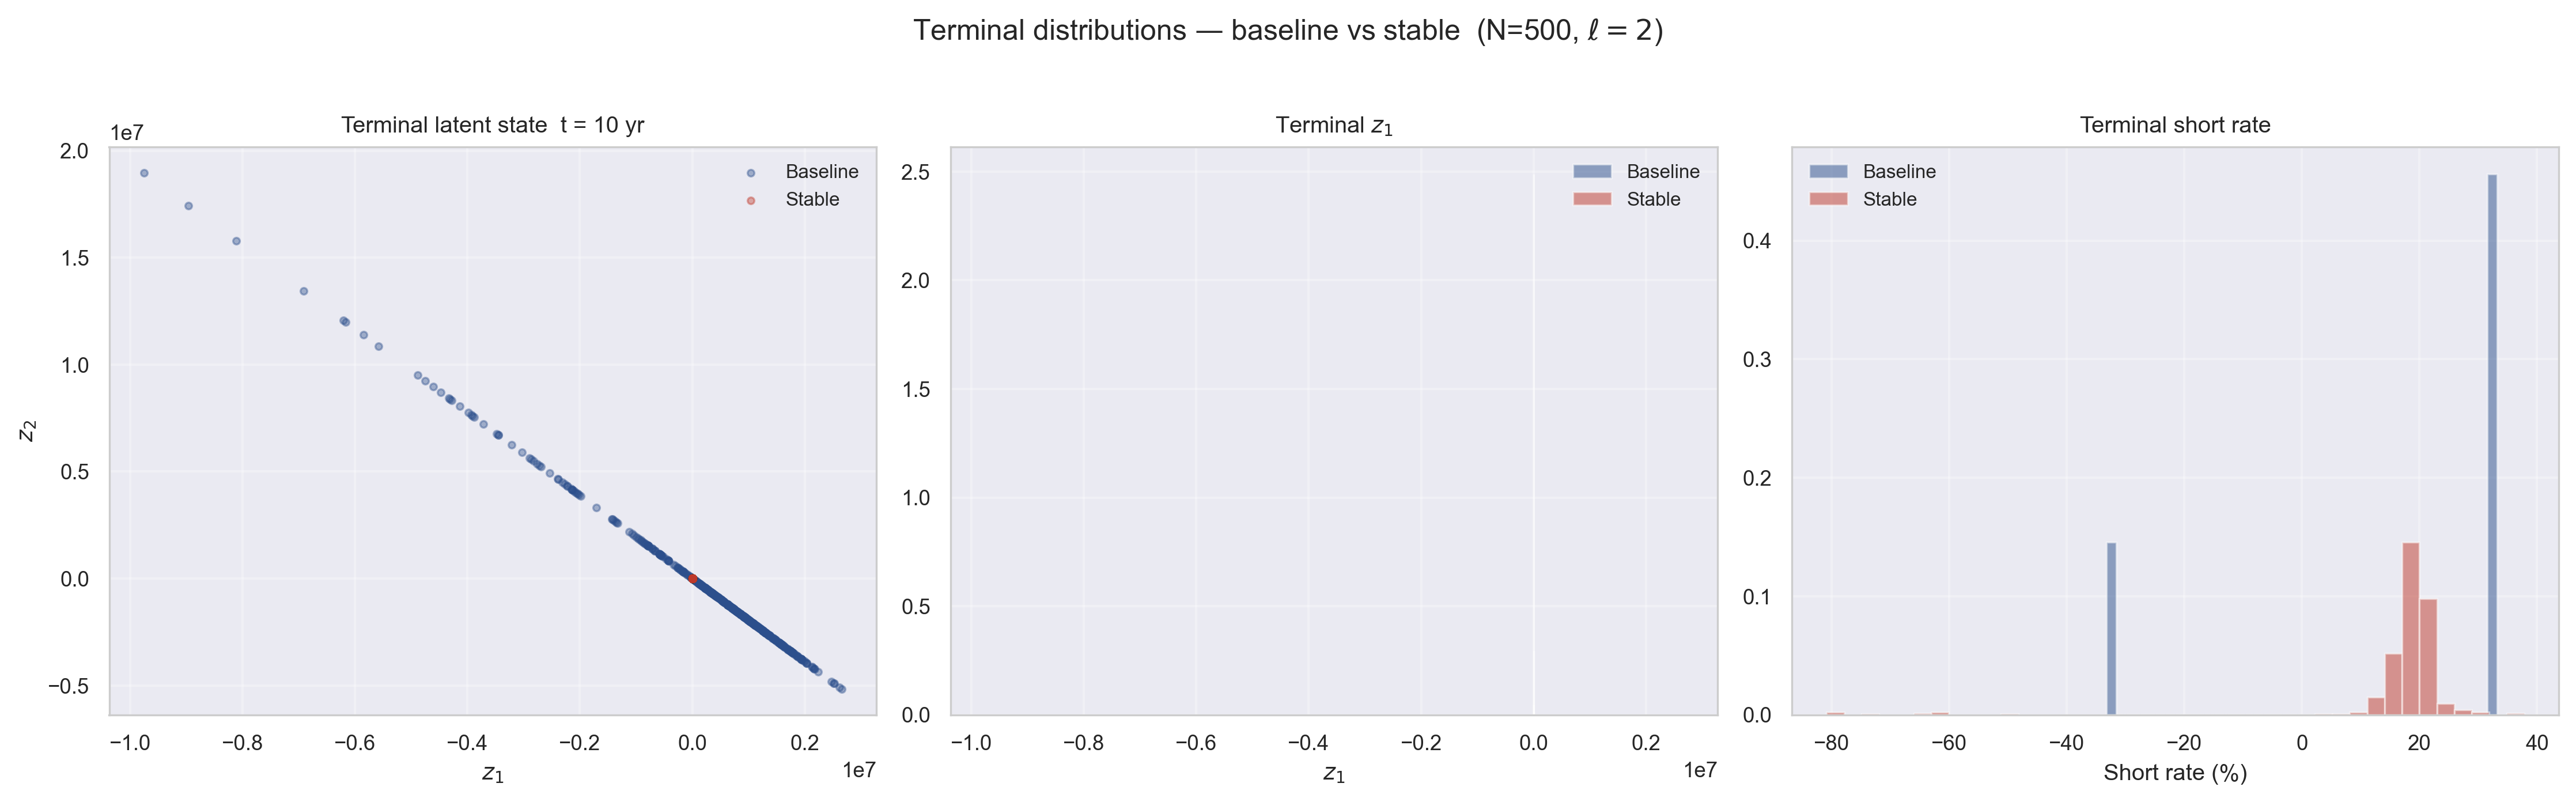
\includegraphics[width=0.85\textwidth]{Figures/Pricing/fig_terminal_dist.png}
    \caption{Terminal latent-state and short-rate distribution at $T_e=2$\,yr for the
    stable ep3500 model (EUR, 500 paths). The compact, near-Gaussian cloud reflects the
    mean-reversion properties established in Chapter~\ref{chap:stable_ae}.}
    \label{fig:terminal_dist}
\end{figure}

\subsection{Swaption Vol Comparison: Pre- and Post-Calibration}
\label{subsec:vol_comparison}

Table~\ref{tab:vol_comparison} provides a template for the swaption normal-vol comparison
produced by \texttt{compare\_swapvol.py}. For each (date, expiry, tenor) triplet the
columns report the market vol, the Stage-1 model vol, and the error in basis points.
The full results are written to the Excel files
\texttt{swaption\_vol\_comparison\_pre\_stage2.xlsx} and
\texttt{swaption\_vol\_comparison\_post\_stage2.xlsx} by \texttt{run\_pricing\_pipeline.py}.

\begin{table}[H]
\centering
\caption{Swaption normal-vol comparison: market vs.\ model (basis points). Rows show
individual (date, expiry × tenor) triplets; the last two rows report MAE and RMSE across
all valid observations.}
\label{tab:vol_comparison}
\begin{tabular}{@{}lrrrrr@{}}
\toprule
Date & $T_e$ & $T_s$ & $\sigma_\mathrm{mkt}$ (bp) & $\hat\sigma_\mathrm{mod}$ (bp) & Error (bp) \\
\midrule
\multicolumn{6}{c}{\textit{[values populated from \texttt{swaption\_vol\_comparison\_pre\_stage2.xlsx}]}} \\
\midrule
\multicolumn{5}{l}{MAE (bp)} & \\
\multicolumn{5}{l}{RMSE (bp)} & \\
\bottomrule
\end{tabular}
\end{table}

\noindent
The percentage of explained vol error removed by the second-stage calibration,
\[
    \text{Improvement} = 1 - \frac{\mathrm{RMSE}_{\mathrm{post}}}{\mathrm{RMSE}_{\mathrm{pre}}},
\]
is the headline metric for assessing the value of the second stage.
